\section{validity confirmation through the Union Bound}
\label{sec4}
%For a given RSC code, the distance spectrum provides information concerning the multiplicity of a codeword for a fixed weight and it is an effective tool to evaluate its error-correcting capability. In practice however, since higher-weight codewords have very little effect on its overall error-correcting capability, we usually use a partial distance spectrum, where the largest codeword weight value is set to $d_{\text{max}}$. 

%The distance spectrum of the RSC code can be obtained from its transfer function, denoted by $$T(Y,X)=\sum_{d=0}^{\infty}\sum_{w=0}^{\infty} a(d,w)Y^dX^w$$ where $a(d,w)$ is the number of codewords of weight $d$ generated by an input bit sequence of weight $w$. 
%The transfer function enumerates all the paths that diverge from and then return to the initial state \cite{ref3}, \textit{i.e.} the RTZ input paths. 
%Once the transfer function of an RSC code is known, it can be used to obtain bounds on the error-correcting capability using the union bound.
%Unfortunately, the complexity involved in deriving the transfer function increases as the number of states of the RSC code increases and other methods such as Mason's Rule \cite{ref3} have to be used. 

%For a given RSC code, we have shown in \ref{subsec:low-weight} that each codeword $c(x)$ is made up of $b(x)$ and $h(x)$ which have $a(x)$ as their common factor as shown in (\ref{novelEq2}) and (\ref{novelEq3}).
 In this section, we obtain a union bound using the low-weight codeword components pattern list and compare it to the union bound obtained via the transfer function as well as simulation results in order to confirm the validity of our proposed method.

To obtain a union bound, let $\cA_h(d)$ be the set of all $a(x)$ which yields weight-$d$ PCs \ie, $w_H(h(x))=w_H(a(x)f(x))=d$ for $a(x) \in \cA_h(d)$. 
Similarly, let $\cA_b(d)$ be the set of all $a(x)$ which yields weight-$d$ SCs \ie, $w_H(b(x))=w_H(a(x)g(x))=d$, for $a(x) \in \cA_b(d)$
while the set of all $a(x)$ which yields weight-$d$ codeword \ie, $w_H(c(x))=w_H(a(x)f(x))+ w_H(a(x)g(x))=d$, is denoted by $\cA_c(d)$.

From \eqref{eq:cw-weight}, when $w_H(b(x)), w_H(h(x)) \geq 2$, we have
\begin{align}
\cA_c(d) = \bigcup_{\ell = 2}^{d-2} \left\{\cA_b(\ell) \cap \cA_h(d-\ell)\right\}
\label{Eq:exactset}
\end{align}
However, to determine $\cA_b(\ell)$ or $\cA_h(\ell)$ for a large $\ell$ is a complex task in general. Thus, in this paper, we replace the set $\cA_c(d)$ by the approximated set $\cA_c'(d)$, written as %\eqref{setApprox}
\begin{equation}
\begin{split}
\cA_c(d) \approx \cA_c'(d) &= \left\{\bigcup_{\ell = 2}^{\ell+1} \left\{\cA_b(\ell) \cap \cA_h(d-\ell)\right\}\right\}\bigcup \left\{\bigcup_{\ell = 2}^{\ell+1} \left\{\cA_b(d-\ell) \cap \cA_h(\ell)\right\}\right\}
\end{split}
\label{setApprox}
\end{equation}
where some codewords in $\cA_c(d)$ with $\ell \approx d-\ell$ may be ignored in $\cA_c'(d)$.
Finally, we obtain the following union bound
\begin{align}
P_b \leq \frac{1}{k} \sum_{d=d_{\text{free}}}^{d_{\text{max}}} \sum_{a(x) \in \cA'_c(d)}w_H(a(x)g(x)) Q\Bigg( \sqrt{\frac{2dE_c}{N_0}}\Bigg)
\label{novelEq7}
\end{align}
where we let $d_{\text{max}}=d_{\text{free}}+3$. 


We verify the validity of our proposed method for the $5/7,~37/21$ and $23/35$ RSC codes, assuming a frame size of $N=64$ is used to obtain the simulation results.
%, we compared the bounds in \eqref{novelEq7} with that obtained using the transfer function method as well as the simulation results for the 
%For each RSC code and a frame size of $N=64$, the codeword is BPSK modulated and transmitted over the AWGN channel. At the receiver end, the Viterbi algorithm is used to decode before a decision is made on the decoded sequence.

\begin{example} {5/7 RSC code}

The polynomial representation of the feedforward and feedback connections for this code are $f(x)=1+x^2$ and $g(x)=1+x+x^2$ respectively. The characteristics of $f(x)$ as well as the low-weight PCs it generates are shown in Example \ref{ex-3} and by multiplying each $a(x)$ by $g(x)$, we obtain the corresponding SCs. On the other hand, the characteristics of $g(x)$ as well as the low-weight SCs are also shown in  Example \ref{ex-1} and the corresponding PCs can be obtained by multiplying each $a(x)$ by $f(x)$.

The SCs and PCs of the 5/7 RSC such that $w_H(b(x))+w_H(h(x)) \leq d_{\text{max}}$ are listed in Table \ref{novelTab13}. 

\begin{table}[htbp]
	\caption{SCs and PCs for the $5/7$ RSC code}
	\centering
	\begin{tabularx}{0.75\textwidth}{Xlll} 
		\hline
		$w_H(c(x))$& $a(x)$ & $b(x)$ & $h(x)$ \\ %[0.5ex] 
		\hline\hline
		5&$1$ & $1+x+x^{2}$ & $1+x^2$\\
		\hline\hline
		6&$1+x^2$ & $1+x+x^3+x^4$ & $1+x^{4}$\\
		%\hline
		&$1+x$ & $1+x^3$ & $1+x+x^2+x^3$\\
		\hline\hline
		&$1+x^2+x^4$ & $1+x+x^3+x^5+x^6$ & $1+x^{6}$\\
		%\hline\hline
		7&$1+x^2+x^3$ & $1+x+x^5$ & $1+x^3+x^4+x^5$\\
		%\hline
		&$1+x+x^2$ & $1+x^2+x^4$ & $1+x+x^3+x^4$\\
		%\hline
		&$1+x+x^3$ & $1+x^4+x^5$ & $1+x+x^2+x^5$\\
		\hline \hline
		8&$1+x^2+x^4+x^6$ & $1+x+x^3+x^5+x^7+x^8$ & $1+x^8$\\
		%\hline
		&$1+x+x^3+x^4$ & $1+x^6$ & $1+x+x^2+x^4+x^5+x^6$\\
		\hline
		%======extra
		%\hline
		%$1+x+x^3+x^5$ & $1+x^4+x^6+x^7$ & $1+x+x^2+x^7$\\
		%\hline
		%$1+x+x^2+x^4$ & $1+x^2+x^5+x^6$ & $1+x+x^3+x^6$\\
		%\hline
		%$1+x+x^2+x^3$ & $1+x^2+x^3+x^5$ & $1+x+x^4+x^5$\\
		%\hline
		%$1+x^2+x^3+x^5$ & $1+x+x^6+x^7$ & $1+x^3+x^4+x^7$\\
		%\hline
		%$1+x^2+x^3+x^4$ & $1+x+x^4+x^6$ & $1+x^3+x^5+x^6$\\
		%\hline
		%$1+x^2+x^4+x^5$ & $1+x+x^3+x^7$ & $1+x^5+x^6+x^7$\\
	\end{tabularx}
	
	\label{novelTab13}
\end{table}

From this table, we observe that every SC such that $w_H(b(x)) >3$ is either a combination of only weight-2 SCs or only weight-3 SCs or both. This means that when this RSC code is used in TC, the deterministic interleaver should be designed in such a way that it deals effectively with weight-2 and weight-3 SCs. While, having to consider weight-3 SCs in the deterministic interleaver design introduces a bit of complexity, it is manageable since there is just a single $(m,n)$ pair that is associated with the weight-3 SCs.

\begin{figure}[htbp]
	\centering
	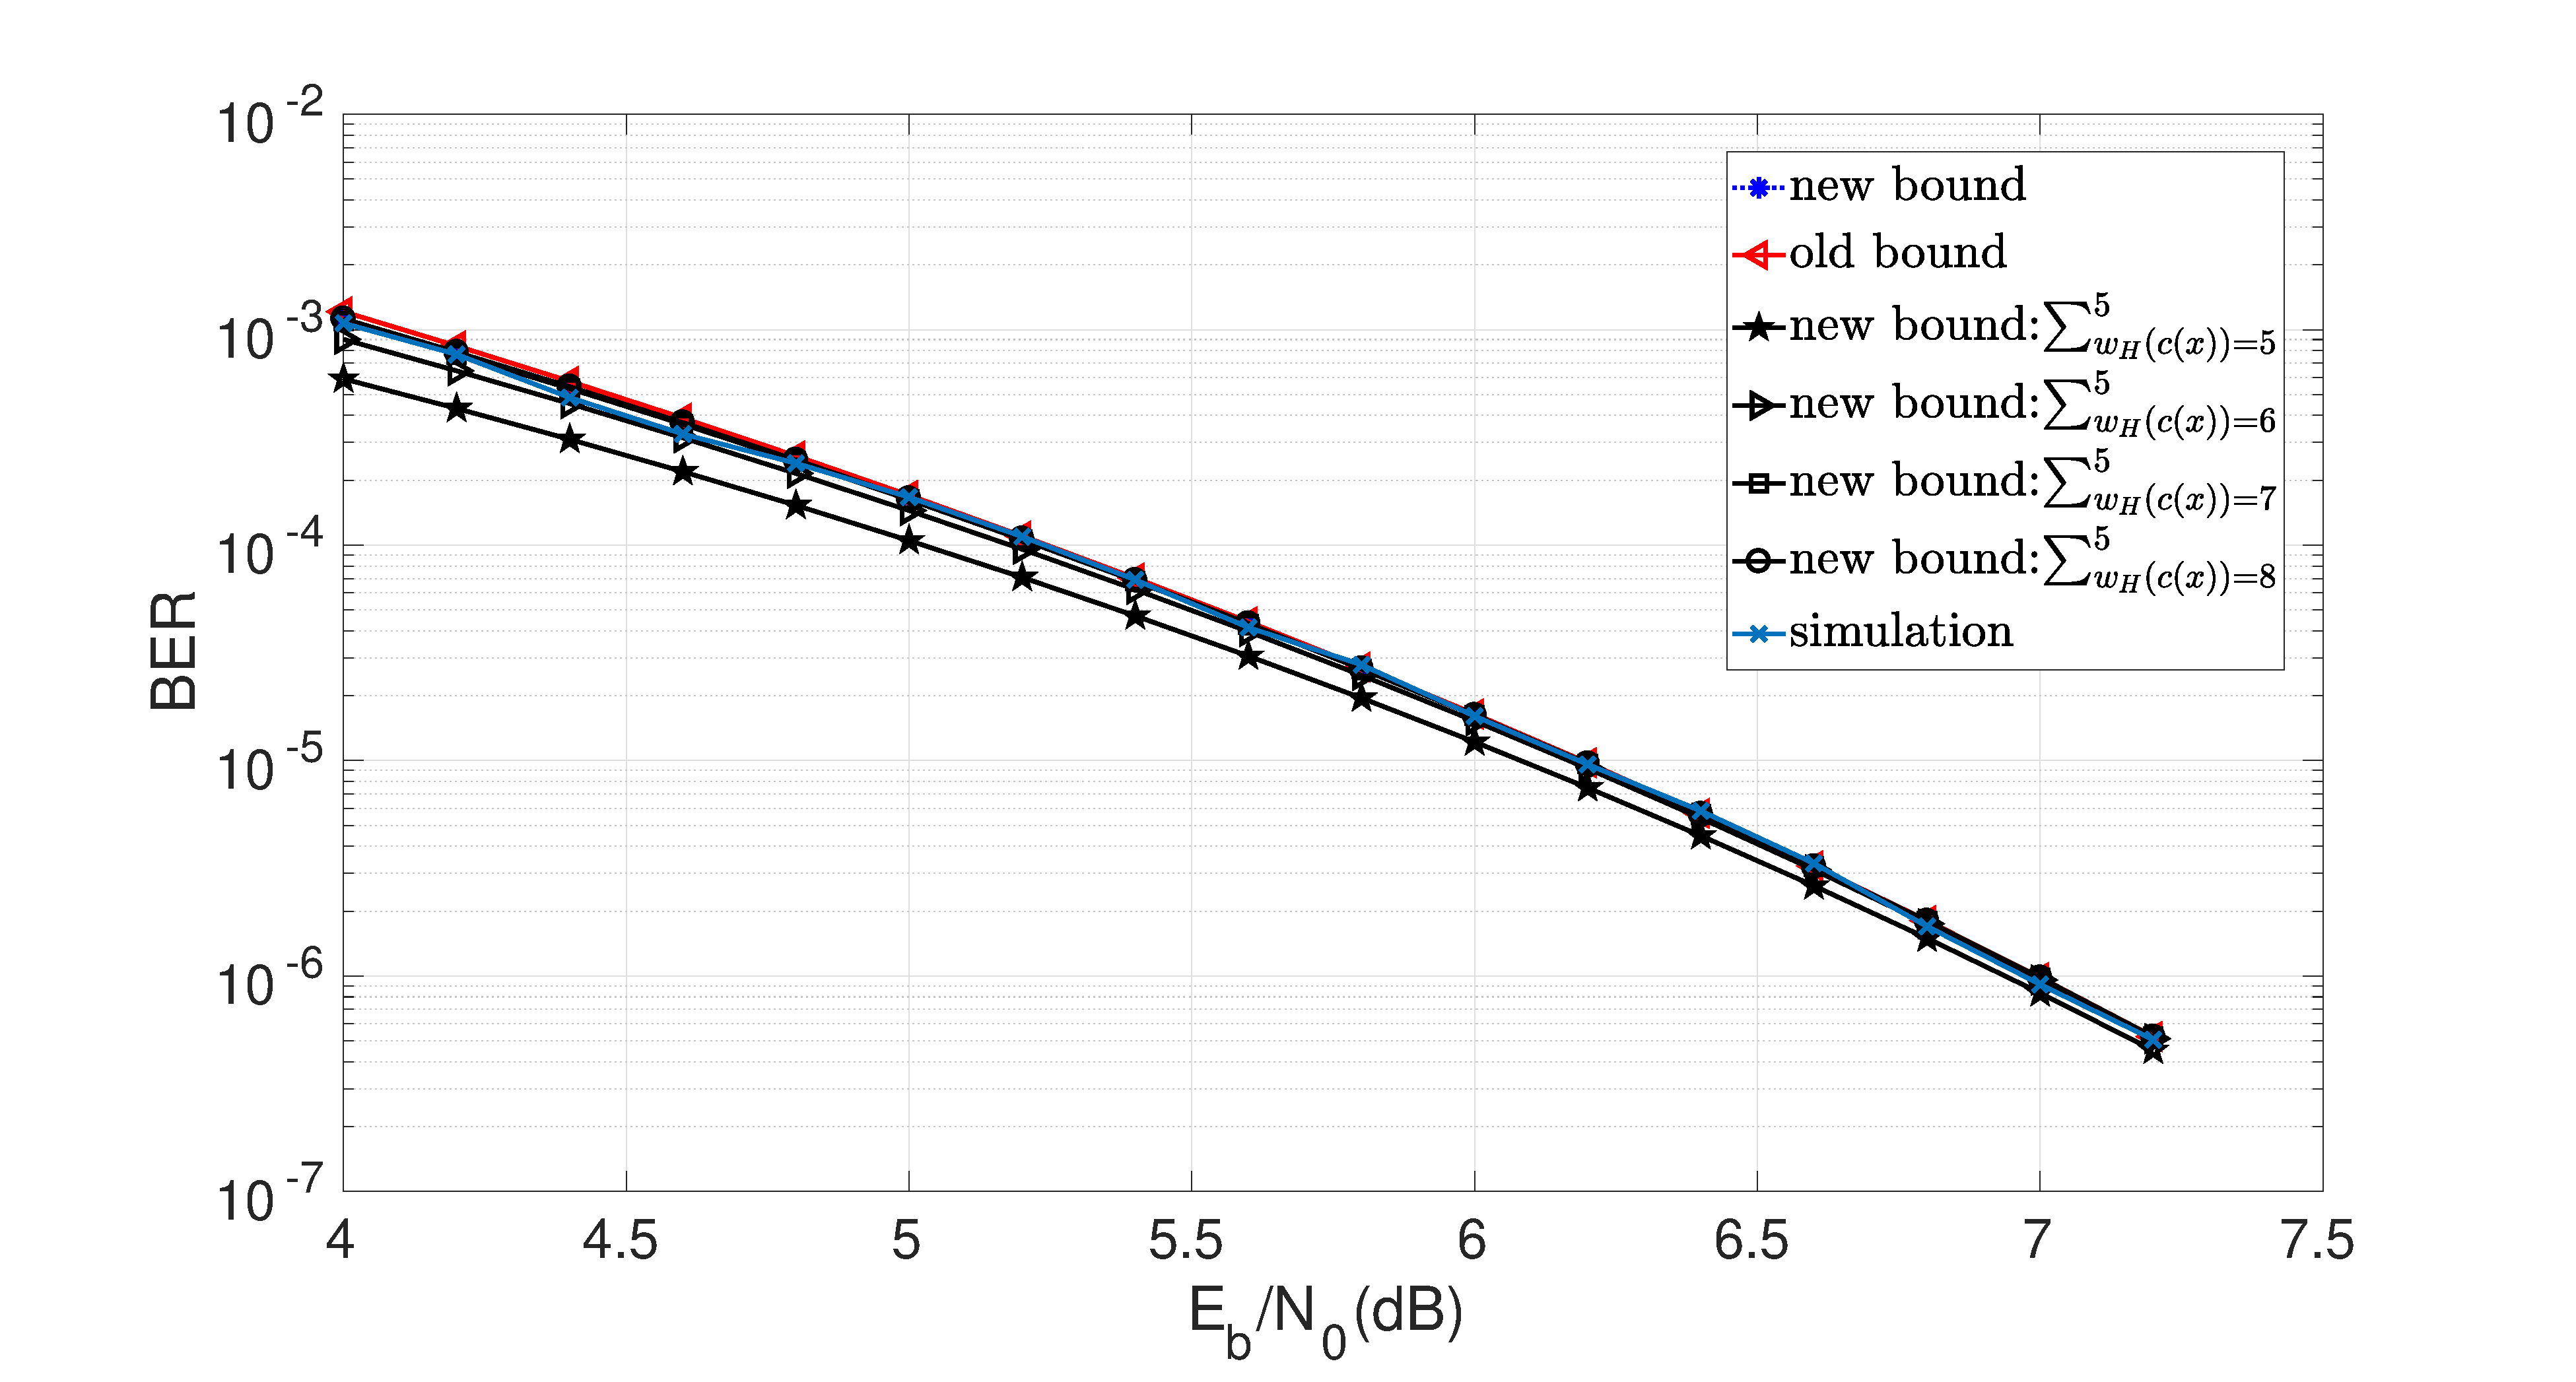
\includegraphics[width=0.5\textwidth]{./Images/RSC_5_7_lower_weights2.eps}
	\captionof{figure}{Old Bound vs New Bound vs Simulation for 5/7 RSC Code}
	\label{simFig1}
\end{figure}

Fig. \ref{simFig1} shows the simulation results for the $5/7$ RSC code as well as the union bound obtained using the transfer function and our proposed method. We can observe that the accuracy of our proposed bound increases with the number of terms used in the approximation. Also, as $E_b/N_0$ increases, the proposed bound as well as the transfer function bound and the simulation results tend to converge. The fact that just a single $(m,n)$ pair needs to be considered for weight-3 SCs during interleaver design makes the 5/7 RSC code attractive for use in TCs.
\label{ex-6}
\end{example}

\begin{example}{37/21 RSC code}

For this code, the feedforward and feedback connections are represented by the polynomials $f(x)=1+x+x^2+x^3+x^4$ and $g(x)=1+x^4$, respectively. The weight-2 and weight-3 SCs and PCs can be obtained by the method demonstrated in Examples \ref{ex-2} and \ref{ex-3}, respectively. The weight-2 and weight-3 SCs and PCs, as well as their corresponding PCs and SCs such that $w_H(b(x))+w_H(h(x)) \leq d_{\text{max}}$ are listed in Table \ref{novelTab14}.
\begin{table}[htbp]
	\caption{SCs and PCs for the $37/21$ RSC code}
	\centering
	\begin{tabularx}{0.75\textwidth}{Xlll} 
		\hline
		$w_H(c(x))$&$a(x)$ & $b(x)$ & $h(x)$ \\ [0.5ex] 
		\hline\hline
		6&$1+x$ & $1+x+x^{4}+x^5$ & $1+x^5$\\
		\hline\hline
		7&$1$ & $1+x^4$ & $1+x+x^2+x^3+x^4$\\
		\hline\hline
		8&$1+x+x^5+x^6$ & $1+x+x^4+x^6+x^9+x^{10}$ & $1+x^{10}$\\
		\hline
		%$1+x+x^4+x^5$ & $1+x+x^8+x^9$ & $1+x^4+x^5+x^9$\\
		%\hline
		%$1+x^2$ & $1+x^2+x^4+x^6$ & $1+x+x^5+x^6$\\
		%\hline
		%$1+x+x^5$ & $1+x+x^4+x^9$ & $1+x^6+x^7+x^8+x^9$\\
		%\hline
		%$1+x+x^4$ & $1+x+x^5+x^8$ & $1+x^4+x^6+x^7+x^8$\\
		%\hline
		%$1+x^2+x^4$ & $1+x^2+x^6+x^8$ & $1+x+x^4+x^7+x^8$\\
		%\hline
		%$1+x^3+x^4$& $1+x^3+x^7+x^8$ & $1+x+x^2+x^4+x^8$\\
		%\hline
		%$1+x^4+x^5$ & $1+x^5+x^8+x^9$ & $1+x+x^2+x^3+x^9$\\
	\end{tabularx}
	
	\label{novelTab14}
\end{table}

From the table, we observe that there are no weight-3 SCs or PCs and every SC such that $w_H(b(x)) > 2$ is a combination of weight-2 SCs. Therefore when this RSC code is used in TCs, the deterministic interleaver needs to be designed to deal with only weight-2 SCs.
\begin{figure}[htbp]
	\centering
	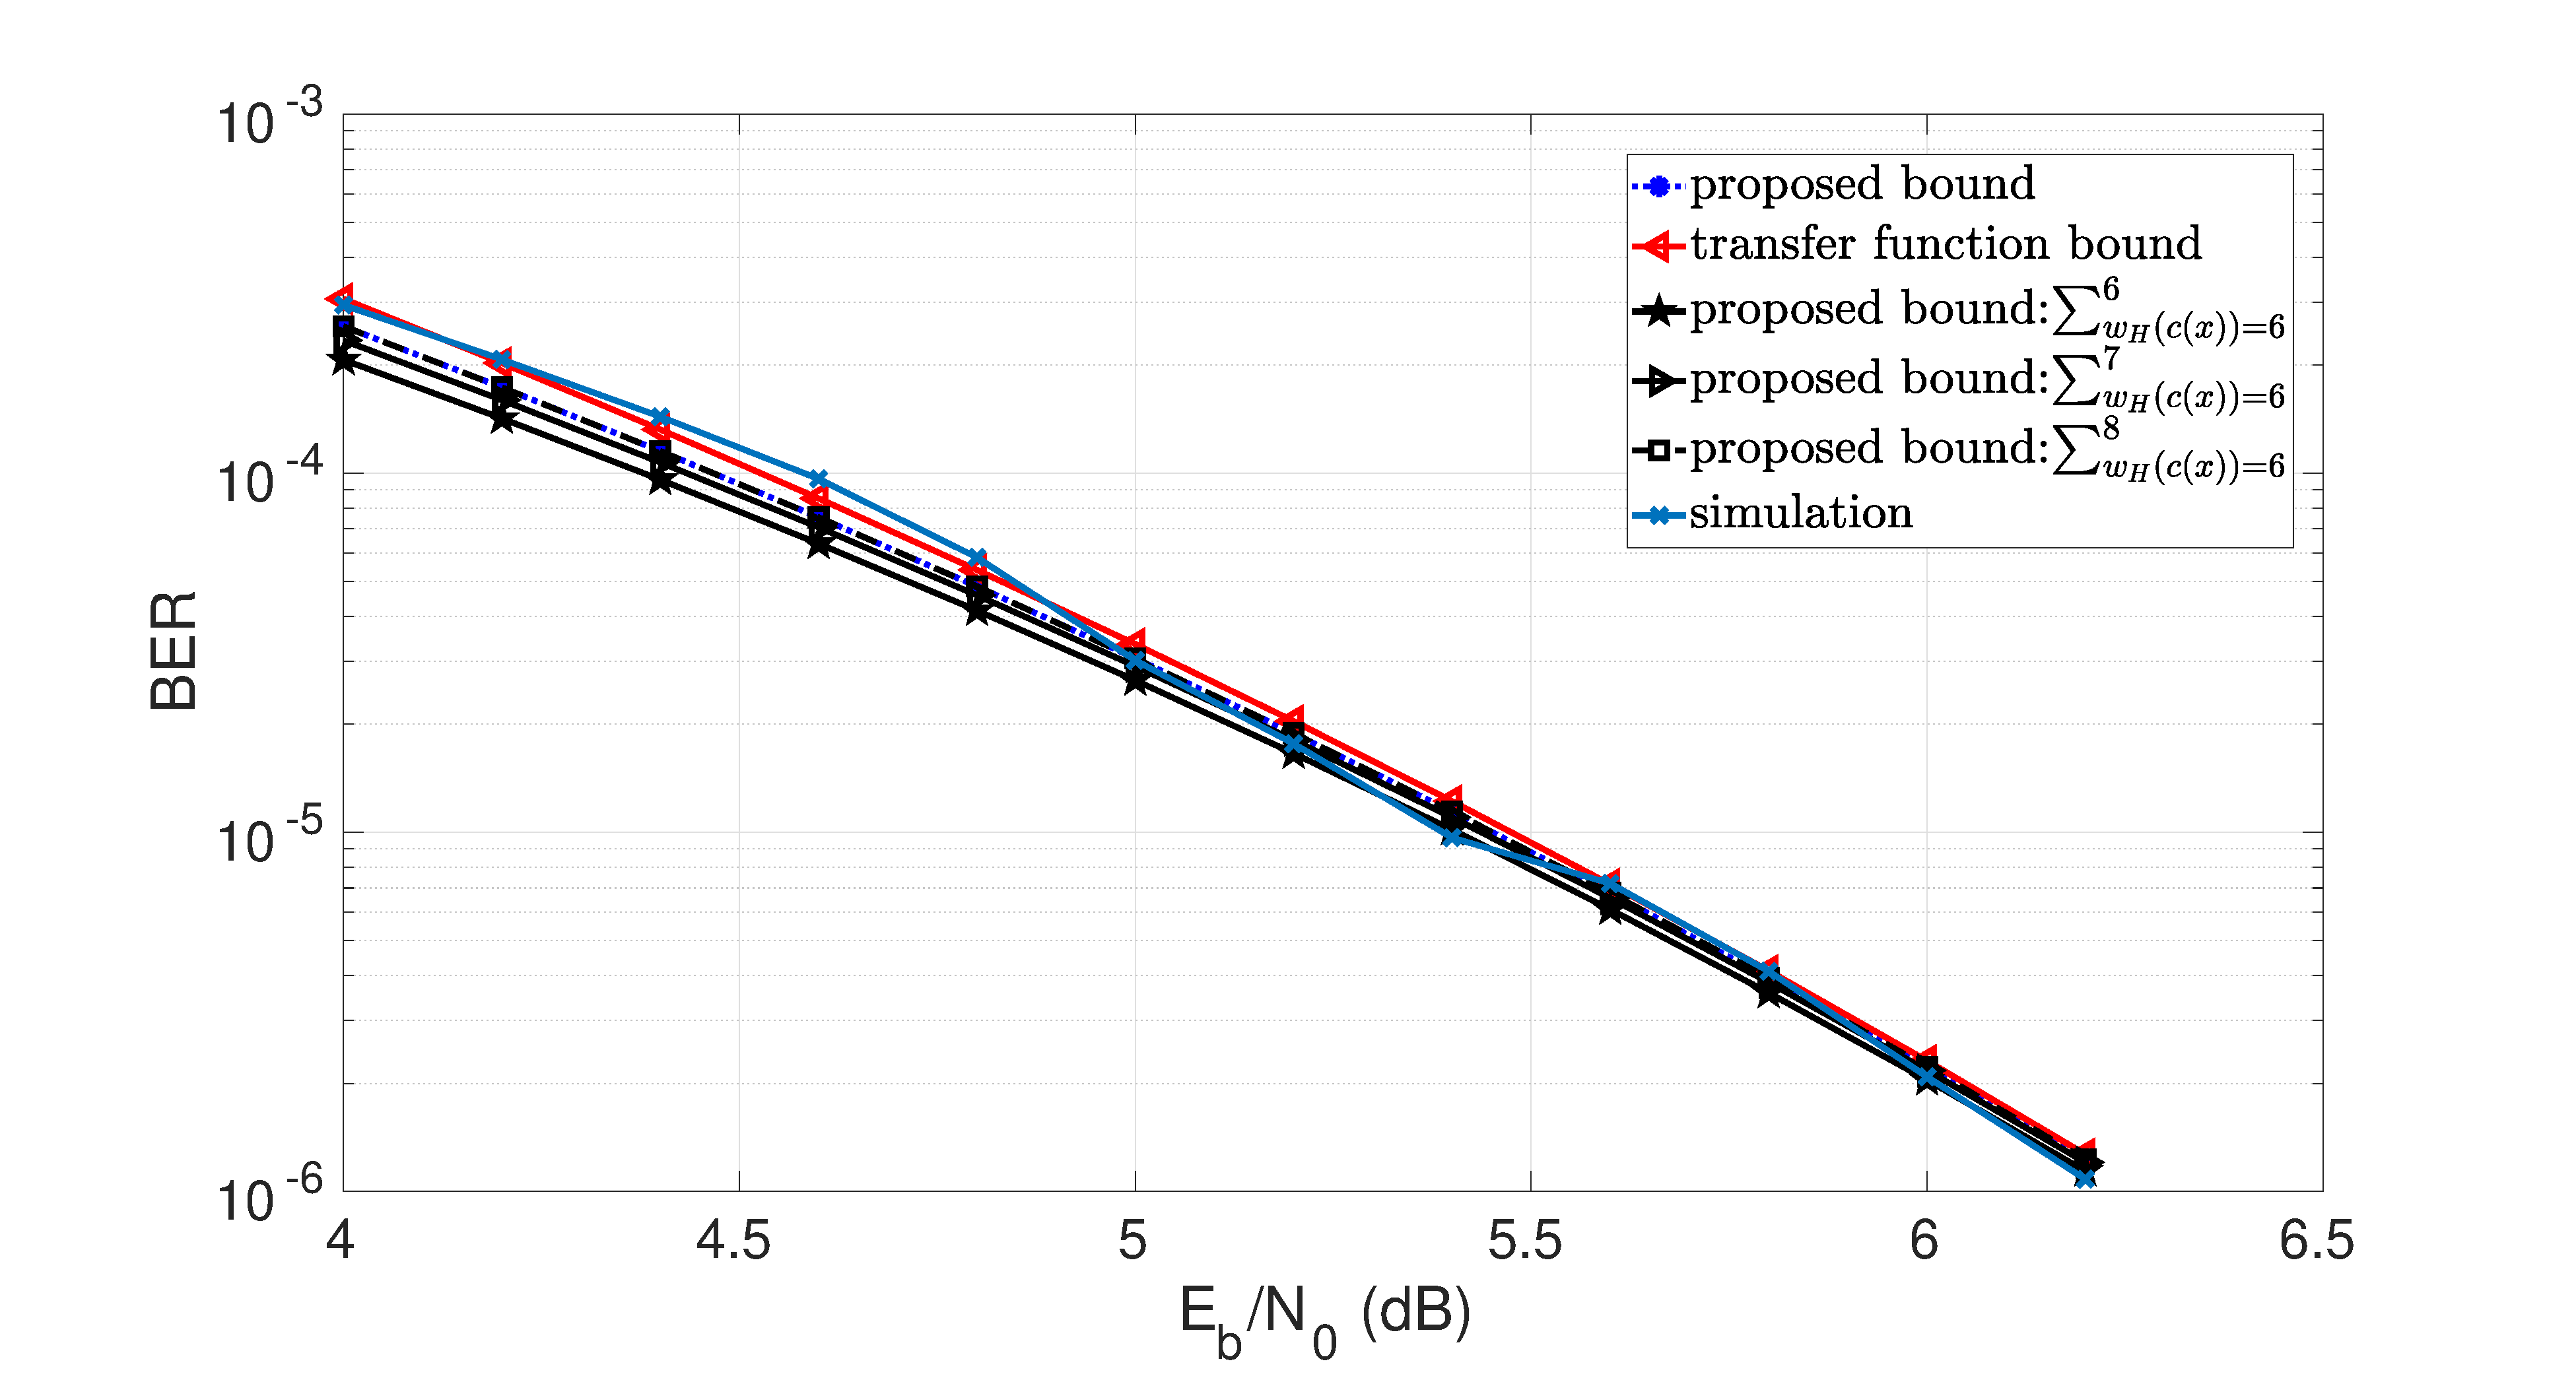
\includegraphics[width=0.5\textwidth]{./Images/RSC_37_21_lower_weights2.eps}
	\caption{Old Bound vs New Bound vs Simulation for 37/21 RSC Code}
	\label{simFig2}
\end{figure}

Fig. \ref{simFig2} shows the simulation results for the $37/21$ RSC code as well as  the transfer function bound and our proposed bound. By observation, we can draw conclusions similar to  Example \ref{ex-6} with respect to the accuracy of our proposed bound . Given that weight-2 SCs and PCs are sufficient to derive the union bound and interleaver design require focusing on weight-2 SCs only, this RSC code is highly recommended for use in TCs.

%, we observe that there is some difference between the new (novel method) bound and the old (transfer function) bound, but they tend to converge as $E_b/N_0$ increases. This suggests that the approximation $ \bigcup_{d = d_{\text{min}}}^{d_{\text{max}}} \cA'_c(d) $ used in our novel method is also sufficient for the $37/21$ RSC code.
%In \ref{simFig3}, we observe that the old bounds and simulation results converge as the Eb/No value increases. However, there is a very distinct gap between the new bound and the old bound. Moreover, the bounds do not converge as the Eb/No increases. This suggests that the approximation used in our novel method is insufficient for this RSC code and considering  $w_H(h(x)),~w_H(b(x))=4$ might yield a more accurate bound.
\label{ex-7}
\end{example}

\begin{example}{$23/35$ RSC code}

The feedforward and feedback connections for this RSC code are represented by the polynomials  $f(x)=1+x+x^4$ and  $g(x)=1+x^2+x^3+x^4$, respectively. The weight-2 and weight-3 PCs can be obtained using the same procedure shown in Example \ref{ex-1}, whiles the weight-2 and weight-3 SCs can be obtained using the same procedure shown in either Example \ref{ex-4} or Example \ref{ex-5}. All SCs and PCs such that $w_H(b(x))+w_H(h(x)) \leq d_{\text{max}}$ are listed Table \ref{novelTab14}.
\begin{table}[htbp]
	\caption{SCs and PCs for the $23/35$ RSC code}
	\centering
	\begin{tabularx}{0.75\textwidth}{lXlX} 
		\hline
		$w_H(c(x))$ & $a(x)$ & $b(x)$ & $h(x)$ \\ [0.5ex] 
		\hline\hline
		7&$1+x^2+x^3$ & $1+x^7$ & $1+x+x^2+x^6+x^7$\\
		\hline
		&$1$ & $1+x^2+x^3+x^4$ & $1+x+x^{4}$\\
		\hline \hline
		9&$1+x+x^2+x^3+x^5$ & $1+x+x^3+x^4+x^8+x^9$ & $1+x^7+x^9$\\
		\hline
		&$1+x+x^2+x^3+x^5+x^7+x^8$ & $1+x+x^3+x^4+x^7+x^{12}$ & $1+x^{11}+x^{12}$\\
		\hline\hline
		10&$1+x^2+x^3+x^7+x^9+x^{10}$ & $1+x^{14}$ & $1+x+x^2+x^6+x^8+x^9+x^{13}+x^{14}$\\
		\hline
	\end{tabularx}
	
	\label{novelTab15}
\end{table}

Similar to Example \ref{ex-7}, there are no weight-3 SCs. However, there exists weight-4 SCs that are not a combination of weight-2 SCs and when this RSC code is used in TCs, the deterministic interleaver needs to be designed to cater for weight-2 SCs as well as such weight-4 SCs. 
 
\begin{figure}[htbp]
	\centering
	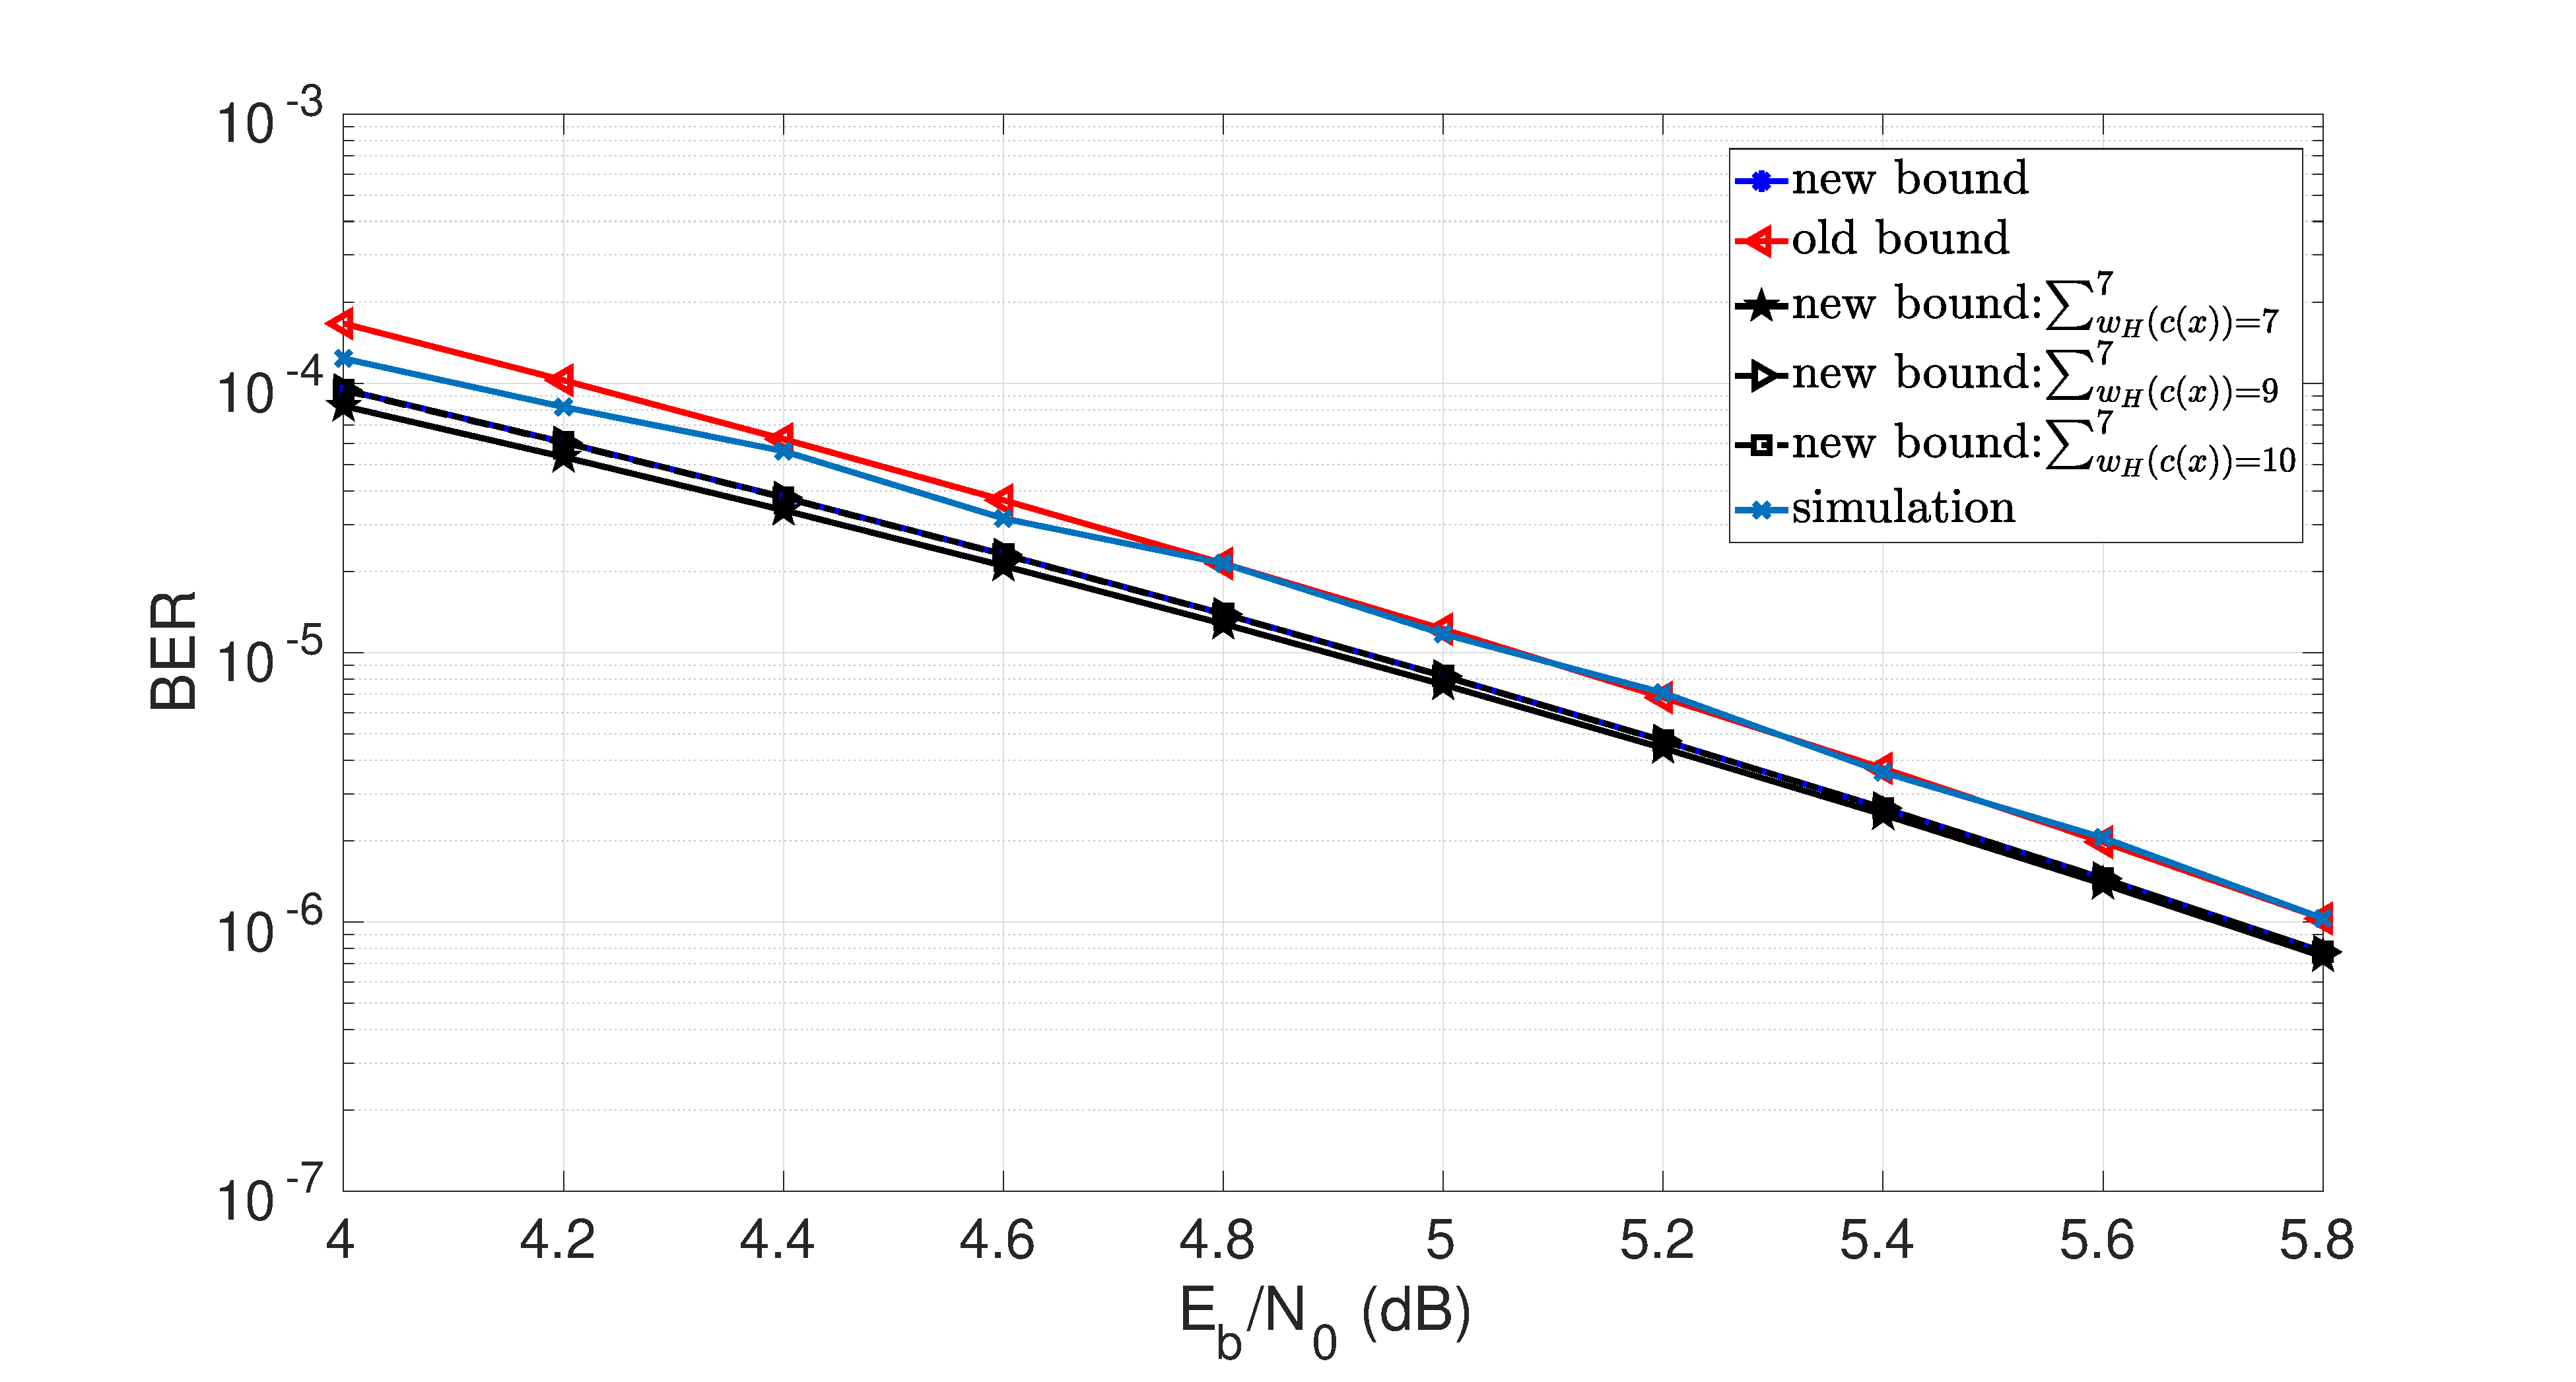
\includegraphics[width=0.5\textwidth]{./Images/RSC_23_35_lower_weights2.eps}
	\caption{Old Bound vs New Bound vs Simulation for 23/35 RSC Code}
	\label{simFig3}
\end{figure}
Fig. \ref{simFig3} shows the simulation results for the $23/35$ RSC code as well as the lower bounds obtained using the transfer function as well as our novel method. Even though the accuracy of our proposed bound increases with the number of terms use, it neither converges with the transfer function bound nor the simulation results as $E_b/N_0$ increases. Even though it is possible to improve the accuracy of our proposed bound by considering SCs and PCs of weight-4, the added complexity as a result of considering weight-4 SCs in the interleaver design process makes this RSC code very unattractive for use in TCs. 
\end{example}

%\begin{figure}[h!]
%\centering
%		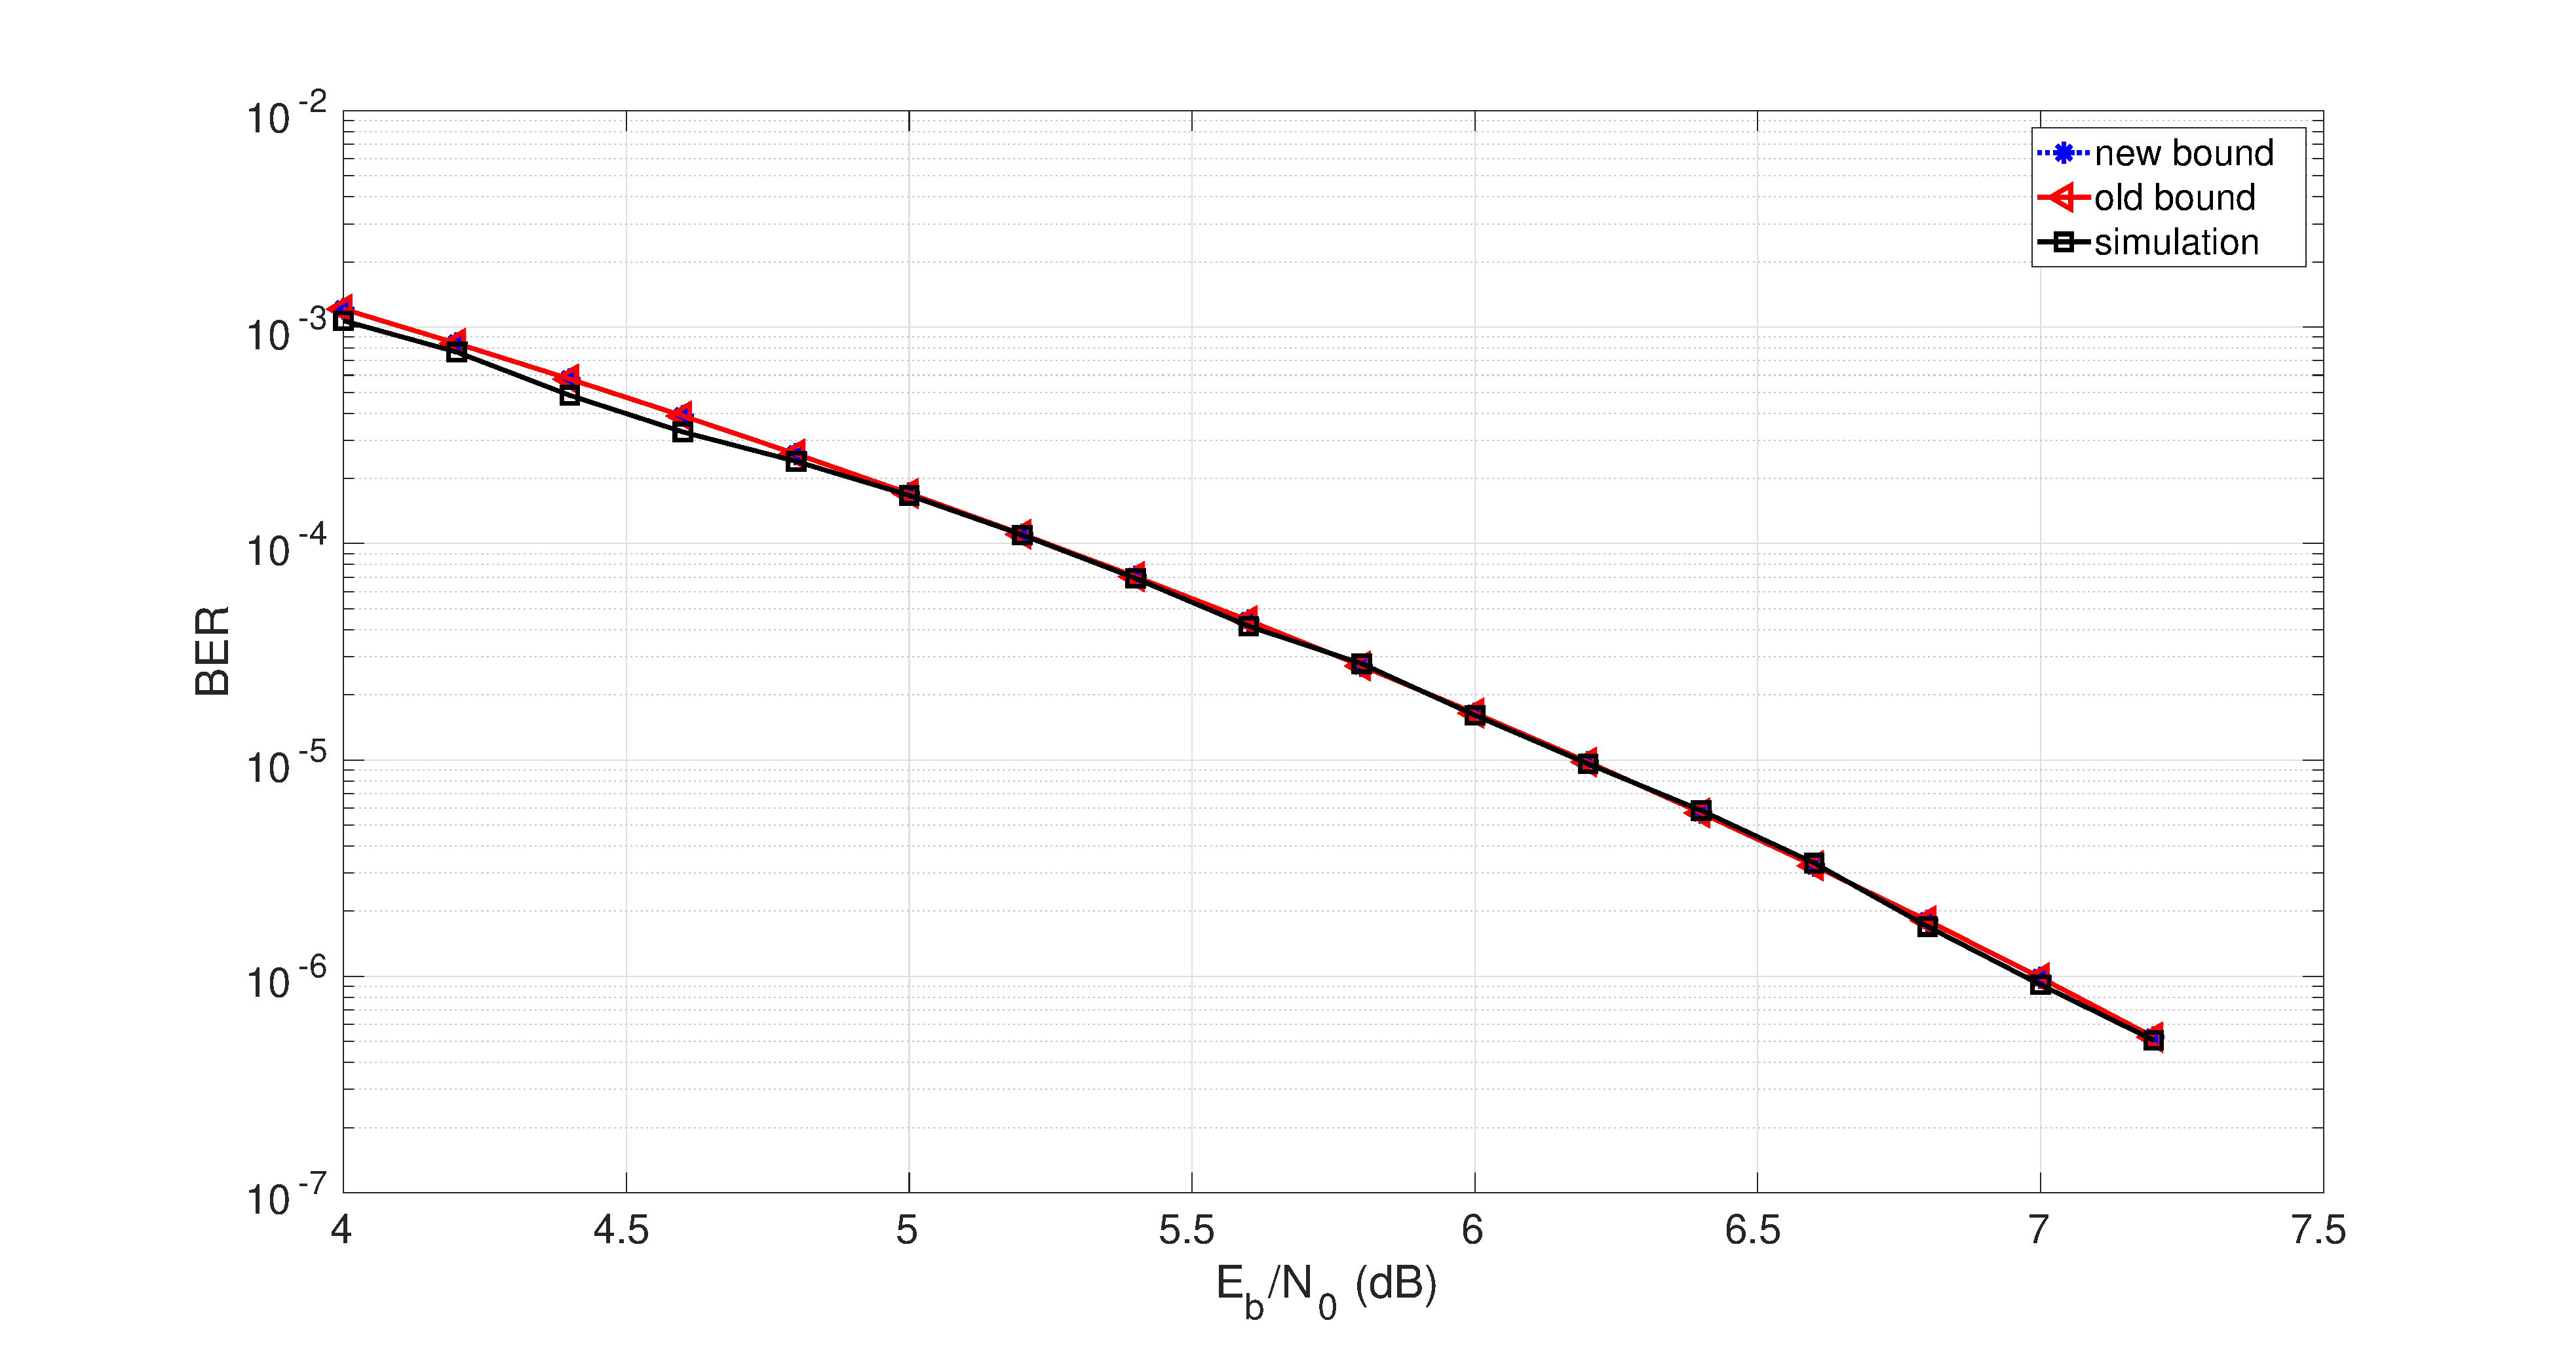
\includegraphics[width=0.8\textwidth]{./Images/RSC_5_7_higher_weights.eps}
%		\caption{Old Bound vs New Bound vs Simulation for 5/7 RSC Code, with higher weights }
%		\label{simFig4}
%		\end{figure}


%		\begin{figure}[h!]
%\centering
%	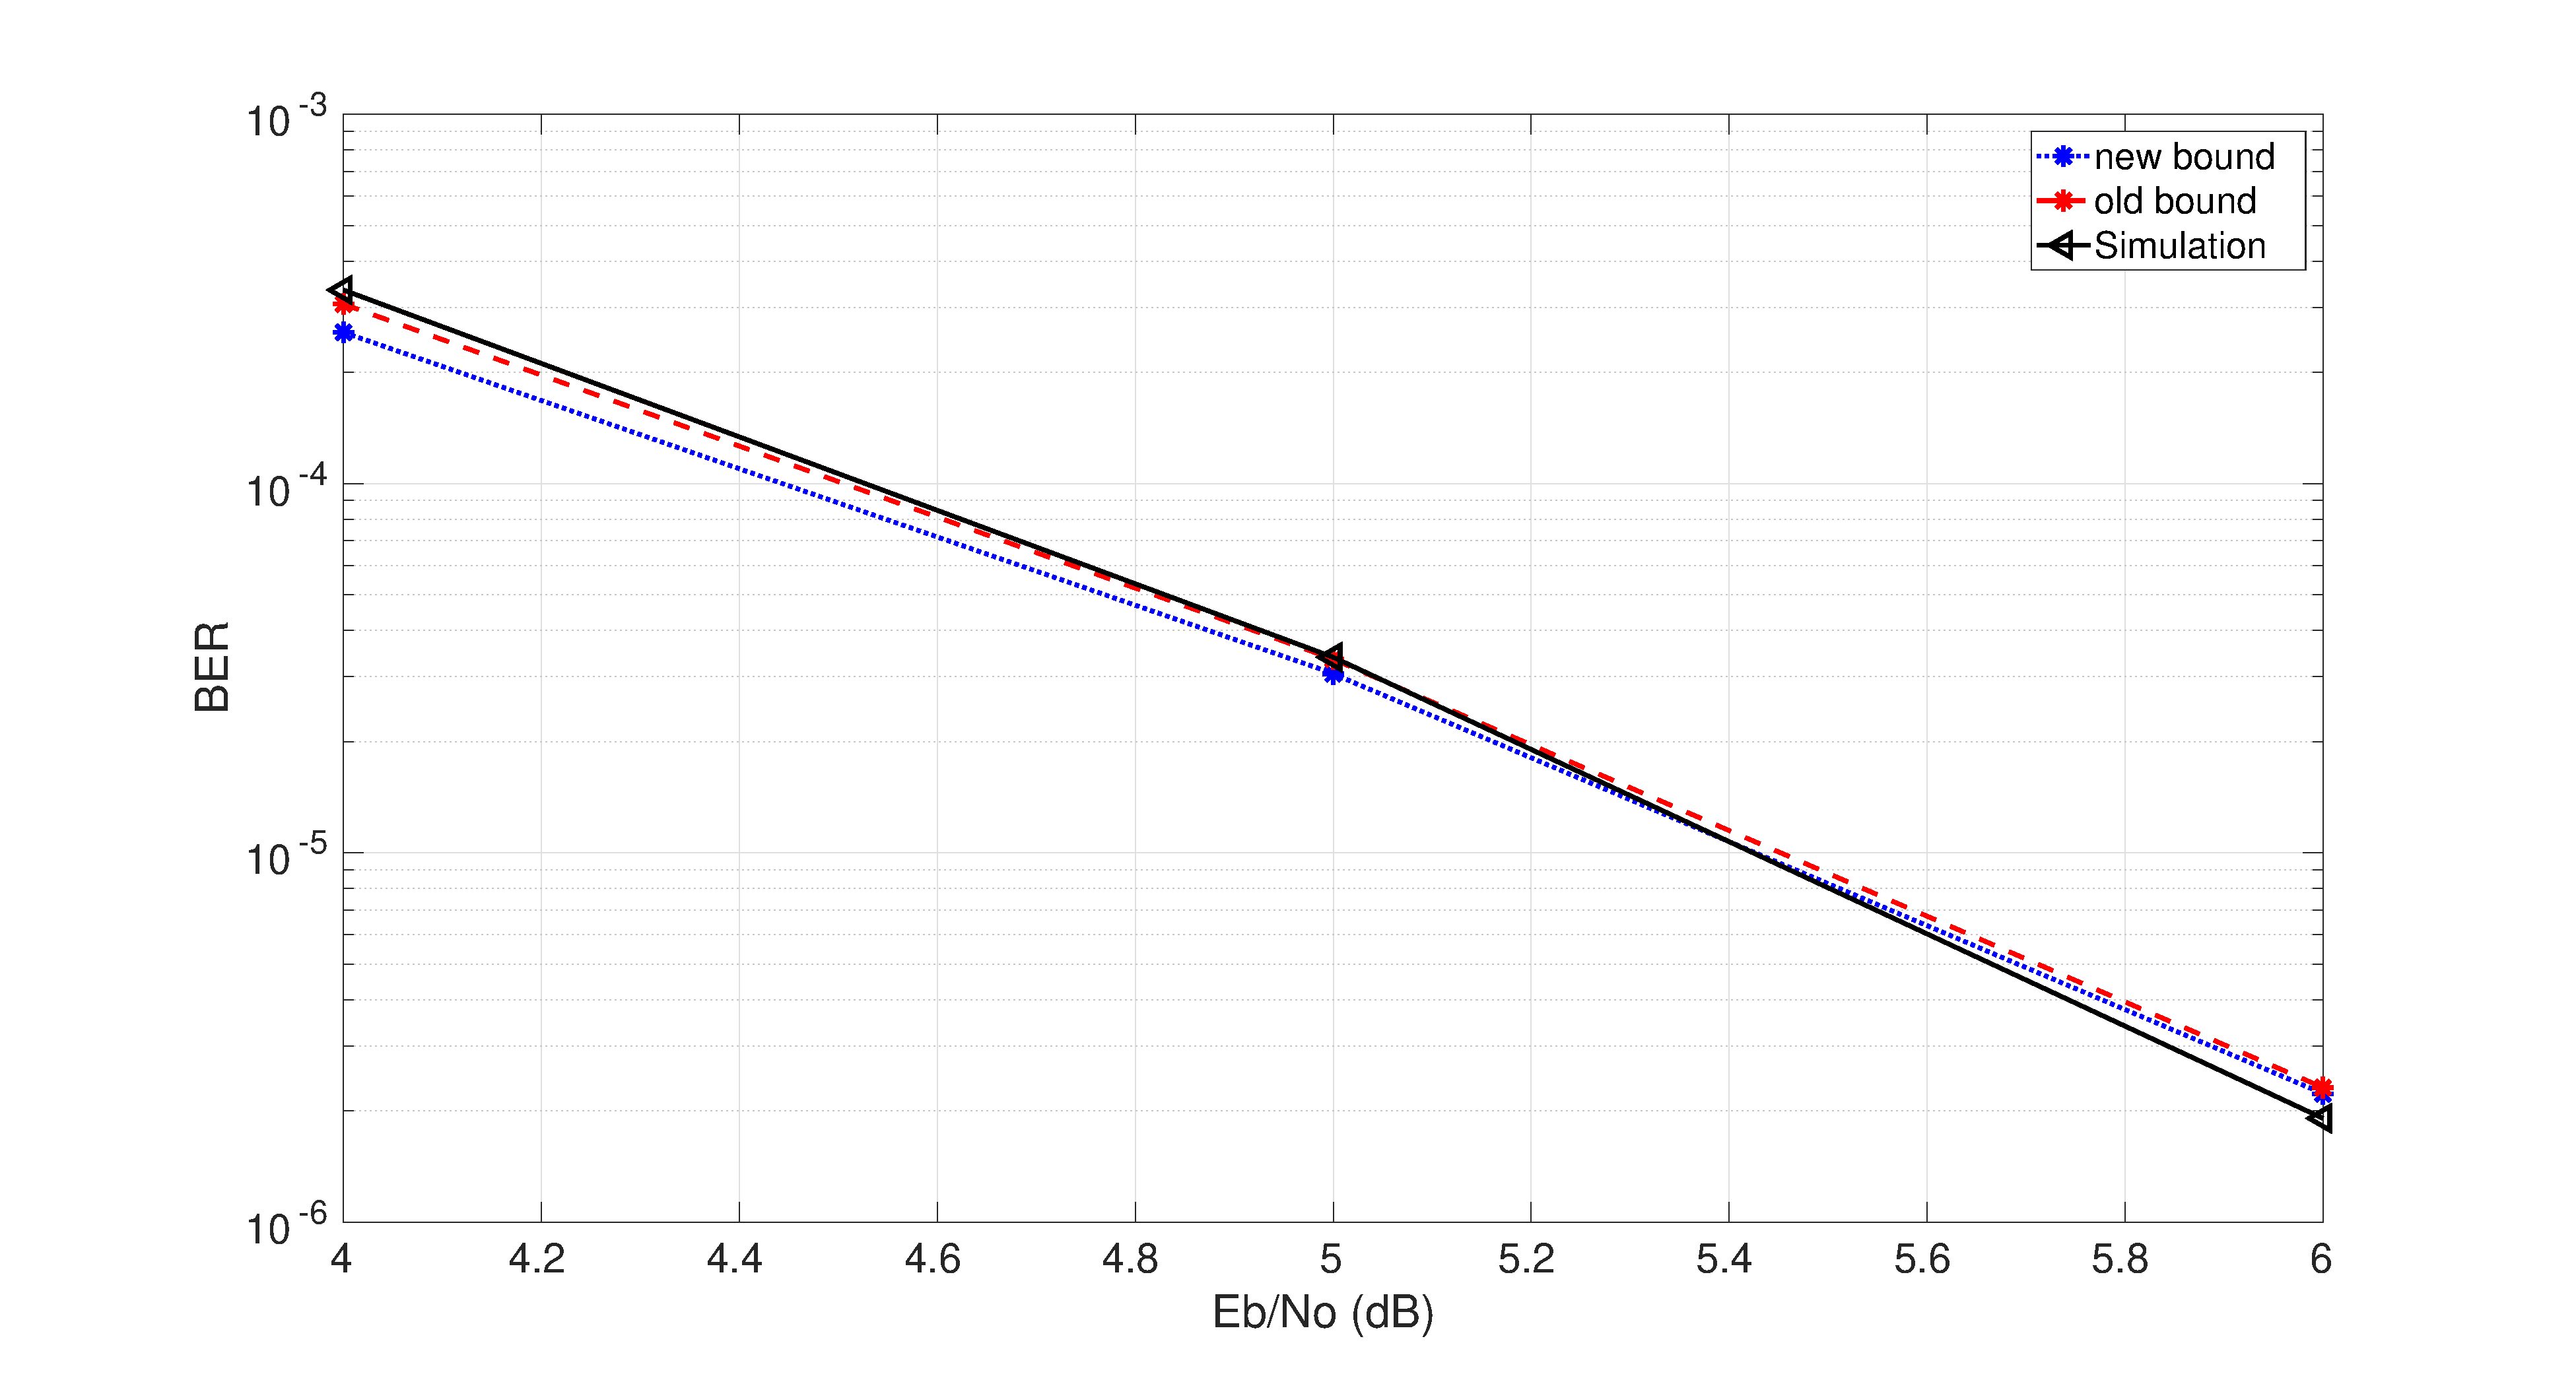
\includegraphics[width=0.5\textwidth]{./Images/RSC_37_21_v2.eps}
%\caption{Old Bound vs New Bound vs Simulation for 37/21 RSC Code, with higher weights}
%\label{simFig5}
%\end{figure}


